\documentclass[letterpaper, 11pt]{scrartcl}
\usepackage{fullpage}
\usepackage{cite}
\usepackage[utf8]{inputenc}
\usepackage{graphicx}
\usepackage[unicode=true,pdfusetitle,
bookmarks=true,bookmarksnumbered=false,bookmarksopen=false,
breaklinks=true,pdfborder={0 0 0},pdfborderstyle={},backref=false,colorlinks=true]
{hyperref}
\hypersetup{linkcolor=blue,citecolor=blue,urlcolor=blue}

%%%%%%%%%%%%%%%%%%%%%%%%%%%%%%%%%%%%%%%%%%%%%%%%%%%%%%%%%%%%%%%%%%%%%%%%%%%%%%%%%%%%%%%%%%%%%%%%%%

\titlehead{Submission for 2020 WPTRC Impact Report\\ \url{https://github.com/aubreymoore/crb-roadside-impact-report/raw/main/main.pdf}}
\title{Using a Cell Phone and Artificial Intelligence to Monitor Coconut Rhinoceros Beetle Damage}
\author{Aubrey Moore}

\begin{document}

\maketitle

Everyone living on Guam has seen damage to coconut palms caused by coconut rhinoceros beetles (CRB). CRB has been on Guam since 2007 \cite{moore2018}. However, until recently, the number of palms being damaged and killed on Guam was unknown. Standardized surveys of CRB damage are needed to monitor changes over time and space, especially in response to control activities and for early detection of CRB in new geographic areas. UOG entomologist Aubrey Moore has developed a highly automated method for routine island-wide monitoring of CRB damage using a cell phone and artificial intelligence.

Only adult rhino beetles cause damage. Grubs feed on decaying vegetation and do no harm. Adult males and females bore into the crowns of coconut palms and other palms to feed on sap. They do not feed on leaves, but they bore holes through developing leaves on their way to the white tissue at the interior of the crown. When these damaged leaves eventually emerge from the crown, they have v-shaped cuts in them, a distinctive sign of CRB damage (Figure \ref{fig:dying_coconuts}). Each adult feeds on sap for only a few days. It then leaves the crown to search for a breeding site. Palms may be killed if a CRB bores through the growing tip (the meristem). Mature palms are rarely killed at low CRB population levels. However, trees are killed when they are simultaneously attacked by many adults during a population outbreak such as the one we are currently experiencing on Guam.

Methods for monitoring CRB damage have been developed. But these rely on direct observation or image analysis by human experts and are too time-consuming and expensive for routine monitoring over large areas. Dr. Trevor Jackson, an entomologist working for AgResearch New Zealand, has developed a survey method based on a five-level scale for classifying CRB damage to individual coconut palms. Jackson's method is being used extensively on CRB-infested islands in the South Pacific. Moore decided to develop an island-wide roadside CRB damage survey for Guam based on an automated version of Jackson's method. 

\section*{Data acquisition} 

In the automated survey, a smart phone mounted on a car or truck records continuous videos of while the vehicle is driven along all major roads on Guam (Figure \ref{fig:mount}). The smart phone uses a couple of free apps: OpenCamera records videos and GPSLogger records GPS coordinates. 

\section*{Data analysis and visualization} 

Analysis of the roadside survey videos is performed by a custom-written Python computer program. This is were artificial intelligence (AI) comes into play. Recent technical breakthroughs in AI have made it much easier to train computers to recognize objects in digital images. Moore collaborated with OnePanel Inc., an AI tech company, to develop and train a couple of object detectors using a technique called \textit{deep learning}.  The first object detector finds all images of coconut palms in the survey videos and classifies each one using Jackson's damage scale. The second object detector locates and counts v-shaped cuts in the fronds of each coconut palm. Data extracted from the videos by the object detectors are saved in a SpatialLite database. To visualize survey results, Moore uses Quantum GIS, to make a publicly available, interactive web map (Figure \ref{fig:webmap}). There are links on the web map to download the survey database and QGIS map project for more detailed analysis (Figure \ref{fig:royal-palms-frame}).  

\section*{Results and discussion}

The first operational island-wide survey on Guam, completed during October 2020, indicated that about 19\% of Guam's coconut palms show CRB damage symptoms. The Guam surveys will be conducted bimonthly. An island-wide roadside video survey is also being done on Rota for early detection of CRB damage.

There is interest in use of roadside video surveys for CRB damage elsewhere in the Pacific and Moore plans to evaluate drone imagery for use on islands without extensive roads. The Guam roadside video survey was designed to be adaptable by using only free open-source software (FOSS) components. Custom-written software for the project as well videos, databases, and GIS projects from surveys will also be made available for download from public repositories hosted on GitHub.

It is interesting to note that this is not the first time that Moore has dabbled with AI. Thirty years ago he trained an artificial neural network to identify free-flying mosquitoes \cite{moore1991}.

\section*{Acknowledgment}

This work is supported by grants from the US Department of the Interior-Office of Insular Affairs, the US Forest Sevice, and USDA-APHIS.  Thanks to UOG entomology technician Christian Cayanan for doing the surveys.

%%%%%%%%%
% FIGURES
%%%%%%%%%

\begin{figure}
	\centering
	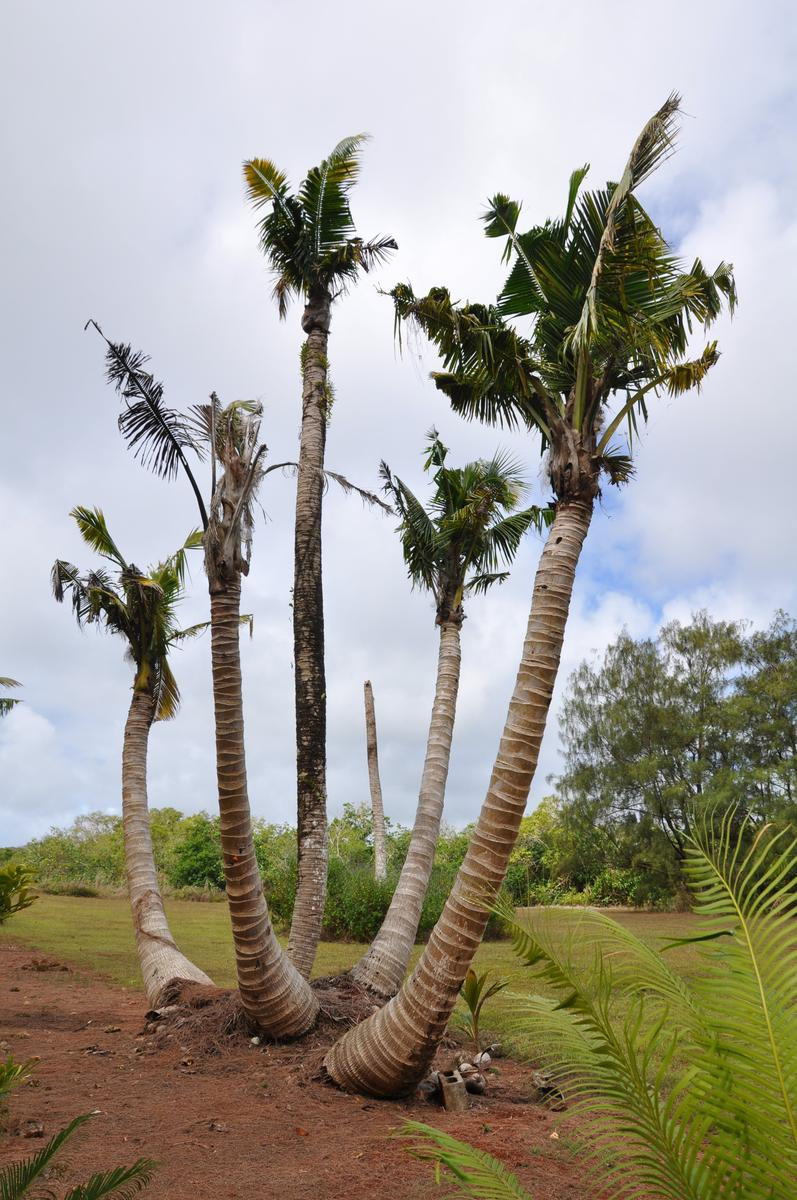
\includegraphics[width=0.8\linewidth]{images/dying_coconuts.png}
	\caption{Coconut palms on Guam damaged by coconut rhinoceros beetle.}
	\label{fig:dying_coconuts}
\end{figure}

\begin{figure}
	\centering
	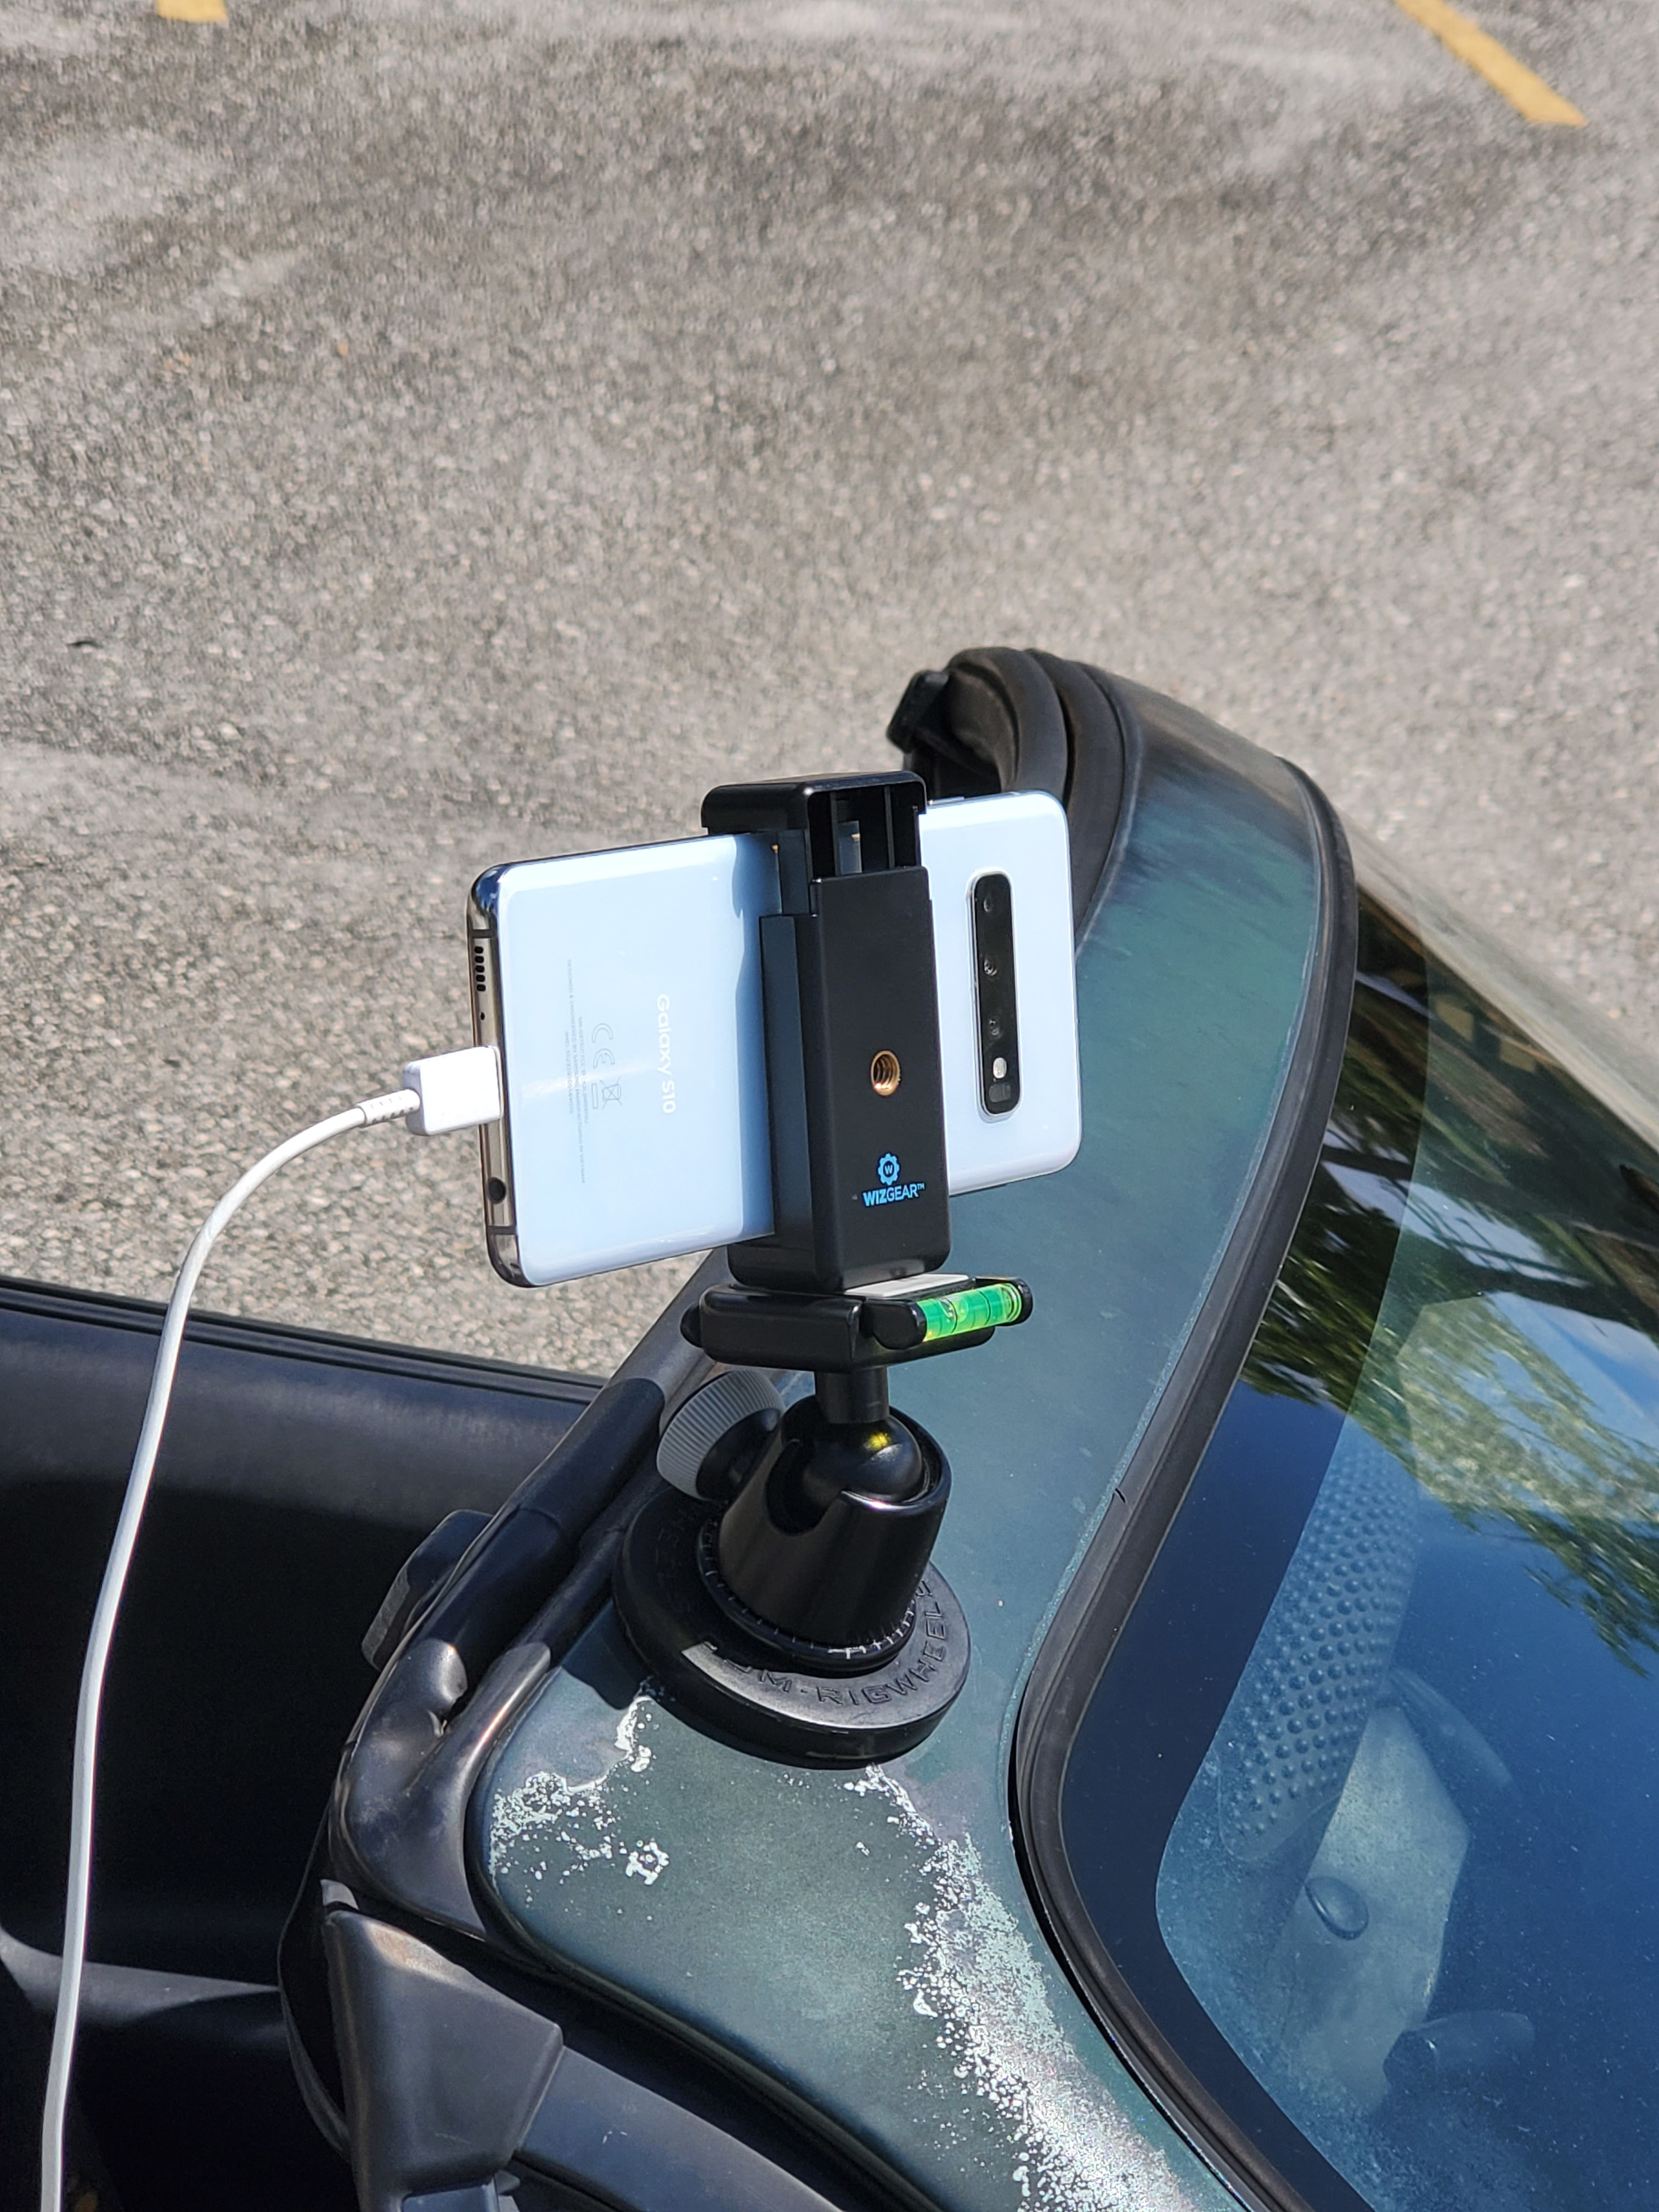
\includegraphics[width=0.9\linewidth]{images/car.jpg}
	\caption{Smart phone attached to a vehicle using a magnetic mount.}
	\label{fig:mount}
\end{figure}

\begin{figure}
	\centering
	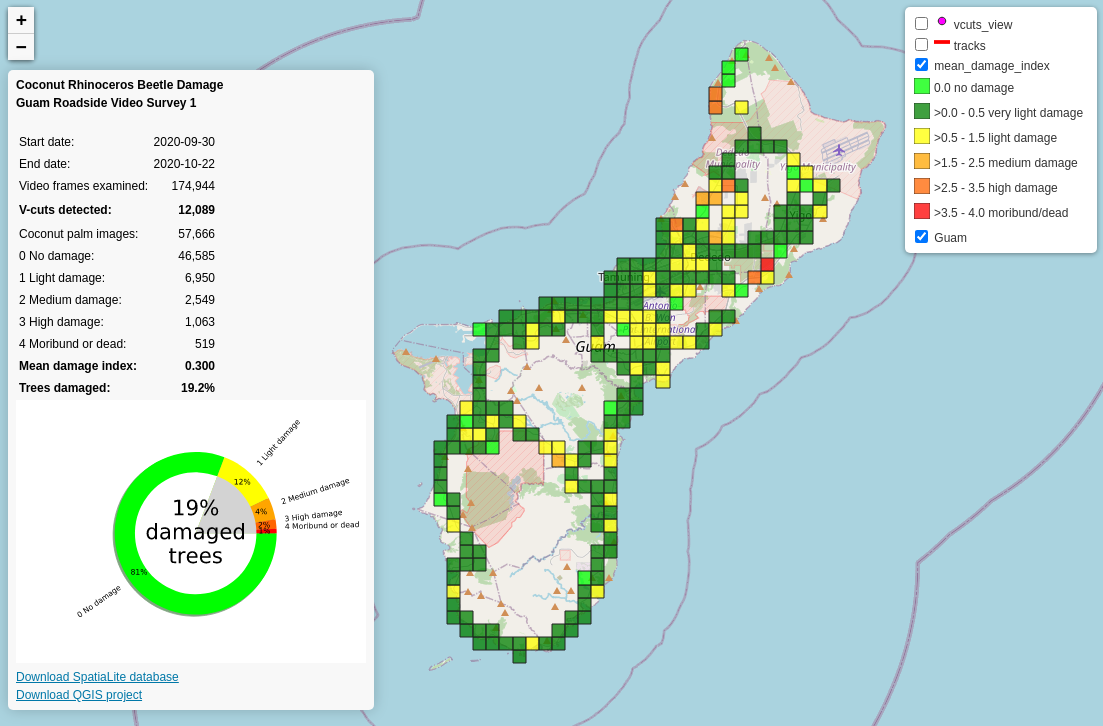
\includegraphics[width=\linewidth]{images/webmap1.png}
	\caption{Interactive web map publicly available at \url{https://aubreymoore.github.io/new-crb-damage-map}.}
	\label{fig:webmap}
\end{figure}

\begin{figure}
	\centering
	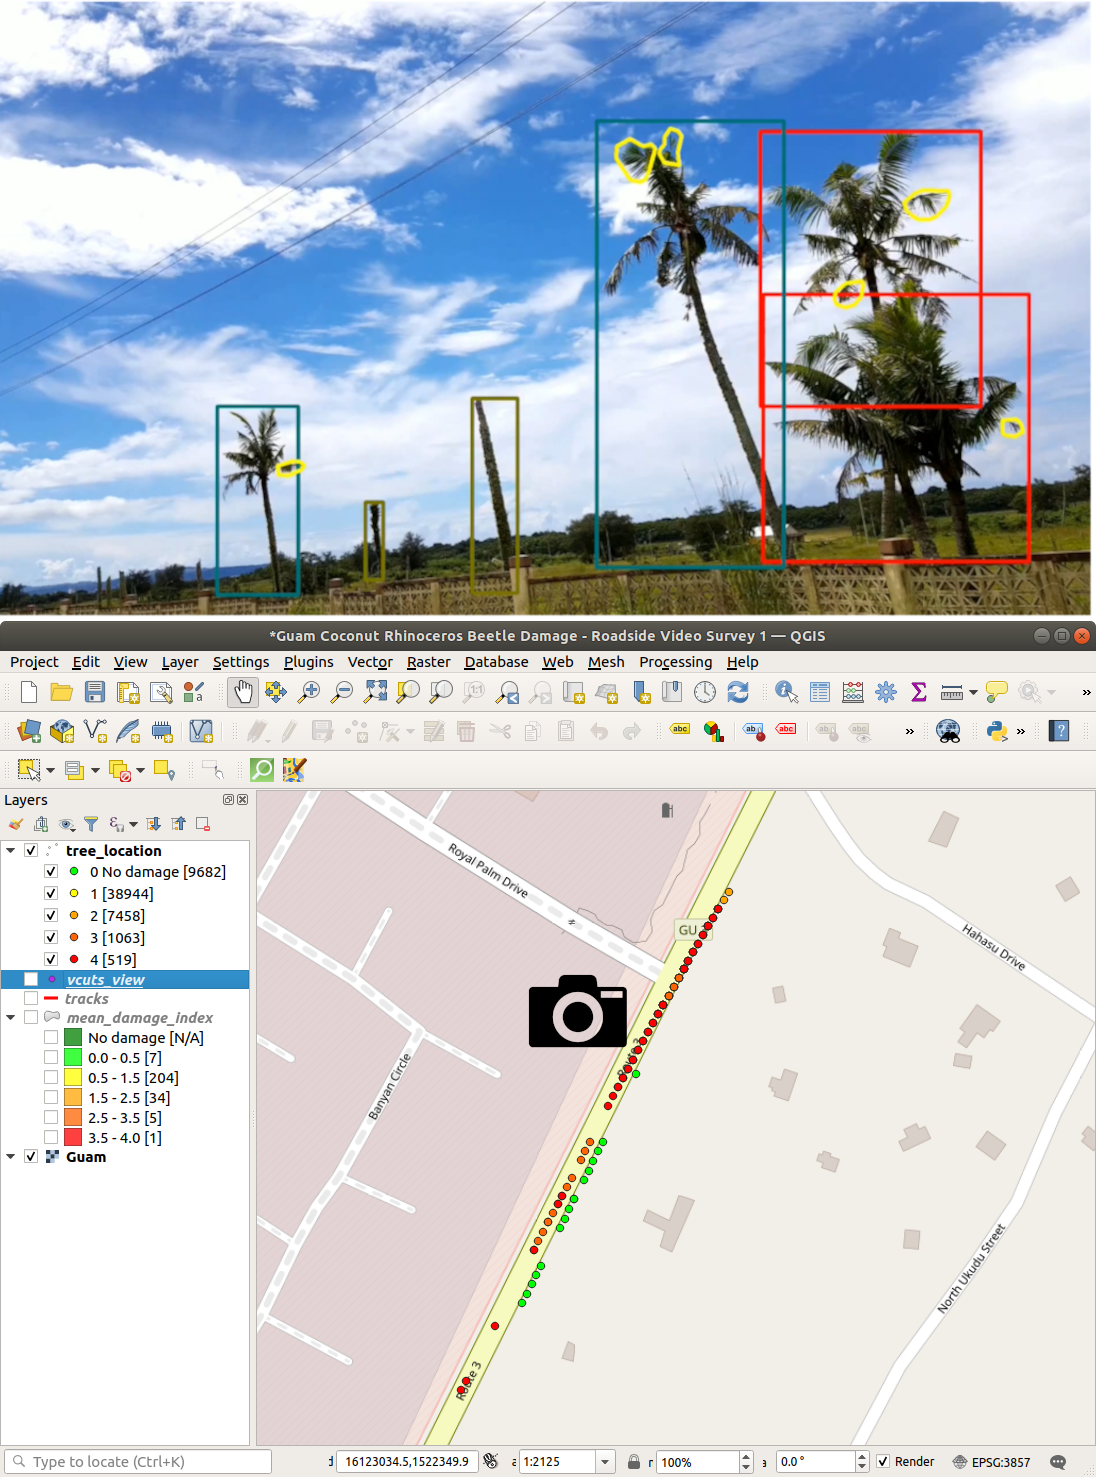
\includegraphics[width=0.8\linewidth]{images/royal-palms-map-framei.png}
	\caption{Medium to severe CRB damage detected in the Royal Palms area of Dededo. Each dot on the map represents a video frame in which one or more coconut palms was detected. The image at the top is a frame extract form a video with approximate at coordinates indicated by the camera icon.}
	\label{fig:royal-palms-frame}
\end{figure}

%%%%%%%%%%%%
% REFERENCES
%%%%%%%%%%%%

\begin{thebibliography}{9}

\bibitem{moore2018}

Moore, Aubrey 2018. The Guam Coconut Rhinoceros Beetle Problem: Past, Present and Future. Zenodo, February 27, 2018. \url{https://doi.org/10.5281/zenodo.1185371}.

\bibitem{moore1991} 
Moore, Aubrey 1991. Artificial neural network trained to identify mosquitoes in flight. Journal of Insect Behavior 4, 391–396.

\end{thebibliography}

\end{document}
